\documentclass[11pt]{article}
\usepackage{fullpage}
\usepackage{authblk}
\usepackage{graphicx}
\usepackage{amsmath}
\usepackage{amsfonts}
\usepackage{amssymb}
\usepackage{amsthm}
\usepackage{mathrsfs}
\usepackage{enumitem}
\usepackage{caption}
\usepackage{subcaption}
\captionsetup{compatibility=false} %This is to fix the issue that 'subcaption' package does not work correctly.

\newtheorem{theorem}{Theorem}%[section]
\newtheorem{lemma}[theorem]{Lemma}
\newtheorem{claim}[theorem]{Claim}
\newtheorem{corollary}[theorem]{Corollary}
\newtheorem{proposition}[theorem]{Proposition}
\newtheorem{definition}[theorem]{Definition}
\newtheorem{remark}[theorem]{Remark}
\newtheorem{assumption}[theorem]{Assumption}
\newtheorem{hypothesis}[theorem]{Hypothesis}
\newtheorem{observation}[theorem]{Observation}

\numberwithin{theorem}{section}

\makeatletter
\renewcommand\section{%
  \@startsection{section}{1}
                {\z@}%
                {-3.5ex \@plus -1ex \@minus -.2ex}%
                {2.3ex \@plus.2ex}%
                {\large\bfseries}% 11pt
}
\renewcommand\subsection{%
  \@startsection{subsection}{2}
                {\z@}%
                {-3.25ex\@plus -1ex \@minus -.2ex}%
                {1sp}% No space after subsections
                {\normalsize\bfseries}% normal size, boldface
}
\renewcommand\subsubsection{%
  \@startsection{subsubsection}{3}
                {\z@}%
                {-3.25ex\@plus -1ex \@minus -.2ex}%
                {1sp}% No space after subsubsections
                {\normalfont\normalsize}% normal size, medium
}
\makeatother

\marginparwidth 0pt \oddsidemargin 0pt \evensidemargin 0pt
\topmargin 30pt \textheight 21.0 truecm \textwidth 16.0 truecm

\title{{\Large\bf  On Kernel Mengerian Orientations of Line Multigraphs}}
\date{}
\author{Han Xiao \footnote{hxiao.math@connect.hku.hk}}

\affil{Department of Mathematics,

The University of Hong Kong,

Hong Kong, China
}


\begin{document}

\numberwithin{equation}{section}

\maketitle
%\thispagestyle{empty}

\openup 1.2\jot

\hfill

\begin{abstract}
We present a polyhedral description of kernels in orientations of line multigraphs.
Given a digraph $D$, let $FK(D)$ denote the fractional kernel polytope defined on $D$,
and let $\sigma(D)$ denote the linear system defining $FK(D)$.
A digraph $D$ is
called kernel perfect if every induced subdigraph $D'$ has a kernel,
called kernel ideal if $FK(D')$ is integral for each induced subdigraph $D'$,
and called kernel Mengerian if $\sigma(D')$ is TDI for each induced subdigraph $D'$.
We show that an orientation of line multigraph is kernel perfect iff it is kernel ideal iff it is kernel Mengerian.
Our result strengthens the theorem of Borodin \textit{et al.} \cite{BoroKost98} on kernel perfect digraphs and generalizes the theorem of Kir\'{a}ly and Pap \cite{KiraPap08} on the stable matching problem.

\hfill

\hfill

\noindent\textbf{AMS subject classifications:} 90C10, 90C27, 90C57.


\noindent\textbf{Key words:} kernel, stable matching, line graph, polytope, total dual integrality.
\end{abstract}


\newpage
\section{Introduction}
\label{intro}
A graph is called \textit{simple} if it contains neither loops nor parallel edges, and is called a \textit{multigraph} if it has parallel edges.
A \textit{simple} digraph is an orientation of simple graph.
A \textit{multi-digraph} is an orientation of multigraph.

Let $G$ be a graph.
The \textit{line graph} of $G$, denoted by $L(G)$, is a graph such that: each vertex of $L(G)$ corresponds to an edge of $G$, and two vertices of $L(G)$ are adjacent if and only if they are incident as edges in $G$.
We call $L(G)$ the \textit{line multigraph} of $G$ if any two vertices of $L(G)$ are connected by as many edges as the number of their common ends in $G$.
We call $G$ a \textit{root} of $L(G)$.

Let $D=(V,A)$ be a digraph.
For $U\subseteq V$, we call $U$ an \textit{independent} set of $D$ if no two vertices in $U$ are connected by an arc, call $U$ a \textit{dominating} set of $D$ if for each vertex $v\not\in U$, there is an arc from $v$ to $U$, and call $U$ a \textit{kernel} of $D$ if it is both independent and dominating.
We call $D$ \textit{kernel perfect} if each of its induced subdigraphs has a kernel.
A \textit{clique} of $D$ is a subset of $V$ such that any two vertices are connected by an arc. We call $D$ \textit{clique-acyclic} if for each clique of $D$ the induced subdigraph of one-way arc is acyclic, and call $D$ \textit{good} if it is clique-acyclic and every directed odd cycle has a (pseudo-)chord\footnote{A pseudo-chord is an arc $(v_i,v_{i-1})$ in a directed cycle $v_1 v_2\ldots v_l v_1$.}.

\begin{theorem}[Borodin \textit{et al.} \cite{BoroKost98}]
\label{thm:BoroKost98}
Let $G$ be a line multigraph. The orientation $D$ of $G$ is kernel perfect if and only if it is good.
\end{theorem}

A subset $P$ of $\mathbb{R}^n$ is called a \textit{polytope} if it is the convex hull of finitely many vectors in $\mathbb{R}^n$. A point $x$ in $P$ is called a \textit{vertex} or an \textit{extreme point} if there exist no distinct points $y$ and $z$ in $P$ such that $x=\alpha y+ (1-\alpha)z$ for $0<\alpha<1$. It is well known that $P$ is the convex hull of its vertices, and that there exists a linear system $Ax\leq b$ such that $P=\{x\in\mathbb{R}^n:Ax\leq b\}$.
We say $P$ is $1/k$-\textit{integral} if its vertices are $1/k$-integral vectors, where $k\in\mathbb{N}$. By a theorem in linear programming, $P$ is $1/k$-integral if and only if $\max\{c^T x:Ax\leq b\}$ has an optimal $1/k$-integral solution for every integral vector $c$ for which the optimum is finite. If, instead, $\max\{c^T x:Ax\leq b\}$ has a dual optimal $1/k$-integral solution, we say $Ax\leq b$ is \textit{totally dual $1/k$-integral} (TDI$/k$).
It is easy to verify that $Ax\leq b$ is TDI$/k$ if and only if $Bx\leq b$ is TDI, where $B=A/k$ and $k\in\mathbb{N}$. Thus from a theorem of Edmonds and Giles \cite{EdmoGile77}, we deduce that if $Ax\leq b$ is TDI$/k$ and $b$ is integral, then $P=\{x\in\mathbb{R}^n:Ax\leq b\}$ is $1/k$-integral.

Let $\sigma(D)$ denote the linear system consisting of the following inequalities:
\begin{alignat}{4}
x(v)+x(N^+(v)) &\geq 1 &\qquad &\forall ~ v~&\in V, \label{domination constraints}\\
x(Q)&\leq 1 &\qquad &\forall ~ Q &\in \mathcal{Q}, \label{independence constraints}\\
x(v) &\geq 0 &\qquad &\forall ~ v~&\in V, \label{vertex nonnegativity}
\end{alignat}
where $x(U)=\sum_{u\in U}x(u)$ for any $U\subseteq V$, $N^+(v)$ denotes the set of all out-neighbors of vertex $v$, and $\mathcal{Q}$ denotes the set of all cliques of $D$. Observe that incidence vectors of kernels of $D$ are precisely integral solutions $x\in \mathbb{Z}^A$ to $\sigma(D)$.
The \textit{kernel polytope} of $D$, denoted by $K(D)$, is the convex hull of incidence vectors of all kernels of $D$.  The \textit{fractional kernel polytope} of $D$, denoted by $FK(D)$, is the set of all solutions $x\in \mathbb{R}^A$ to $\sigma(D)$. Clearly, $K(D)\subseteq FK(D)$.
We call $D$ \textit{kernel ideal} if $FK(D')$ is integral for each induced subdigraph $D'$, and \textit{kernel Mengerian} if $\sigma(D')$ is TDI for each induced subdigraph $D'$.

As described in Egres Open \cite{Egres}, the polyhedral description of kernels remains open. Chen \textit{et al.} \cite{ChenChen} attained a polyhedral characterization of kernels by replacing clique constraints $x(Q)\leq 1$ for $Q\in\mathcal{Q}$ with independence constraints $x(u)+x(v)\leq 1$ for $(u,v)\in A$.
In this paper we show that kernels in orientations of line multigraph can be characterized polyhedrally.

\begin{theorem}
\label{thm:main}
Let $D$ be an orientation of a line multigraph. Then the following statements are equivalent:
\begin{enumerate}[label={\emph{(}\roman*\emph{)}}]
	\item $D$ is good;
	\item $D$ is kernel perfect;
	\item $D$ is kernel ideal;
	\item $D$ is kernel Mengerian.
\end{enumerate}
\end{theorem}

The equivalence of $(i)$ and $(ii)$ was established by Borodin \textit{et al.} \cite{BoroKost98} (Maffray \cite{Maff92} proved the case when $D$ is perfect). Kir\'{a}ly and Pap \cite{KiraPap08} proved Theorem \ref{thm:main} for the case when the root of $D$ is bipartite.
Our result strengthens the theorem of Borodin \textit{et al.} \cite{BoroKost98} and generalizes the theorem of Kir\'{a}ly and Pap \cite{KiraPap08} to line multigraphs.


\section{Preliminaries}
\label{pre}
Kernels are closely related to stable matchings.
Before proceeding, we introduce some notations and some theorems of the stable matching problem first.
Let $G=(V,E)$ be a graph.
For $v\in V$, let $\delta(v)$ denote the set of edges incident to $v$ and $\prec_v$ be a strict linear order on $\delta(v)$.
We call $\prec_v$ the \emph{preference} of $v$, and for edges $e$ and $f$ incident to $v$ we say $v$ \emph{prefers} $e$ to $f$ or $e$ \emph{dominates} $f$ if $e\prec_v f$.
Let $\prec$ be the set of linear order $\prec_v$ for $v\in V$.
We call the pair $(G,\prec)$ \emph{preference system}, and call $(G,\prec)$ \emph{simple} if $G$ is simple.
For $e\in E$, let $\varphi(e)$ denote the set consisting of $e$ itself and edges that dominate $e$ in $(G,\prec)$,
and let $\varphi_v(e)$ denote the set of edges that dominate $e$ at vertex $v$ in $(G,\prec)$.
Given a matching $M$ in $G$, we call $M$ \emph{stable} in $(G,\prec)$ if every edge of $G$ is either in $M$ or is dominated by some edge in $M$.

Let $\pi(G,\prec)$ denote the linear system consisting of the following linear inequalities:
\begin{alignat}{3}
x(\varphi(e)) &\geq 1 &\qquad \forall ~e &\in E,\label{stability constraints}\\
x(\delta(v)) &\leq 1 &\qquad \forall ~v &\in V,\label{matching constraints}\\
x(e) &\geq 0 &\qquad \forall ~e &\in E.\label{edge nonnegativity}
\end{alignat}
As observed by Abeledo and Rothblum \cite{AbelRoth94}, incidence vectors of stable matchings of $(G,\prec)$ are precisely integral solutions $x\in \mathbb{Z}^E$ to $\pi(G,\prec)$.
The \textit{stable matching polytope}, denoted by $SM(G,\prec)$, is the convex hull of incidence vectors of all stable matchings of $(G,\prec)$. The \textit{fractional stable matching polytope}, denoted by $FSM(G,\prec)$, is the set of all solutions $x\in \mathbb{R}^E$ to $\pi(G,\prec)$. Clearly, $SM(G,\prec)\subseteq FSM(G,\prec)$.

\begin{theorem}[Rothblum \cite{Roth92}]
\label{thm:Roth92}
Let $(G,\prec)$ be a simple preference system. If $G$ is bipartite, then
$SM(G,\prec)=FSM(G,\prec)$.
\end{theorem}

\begin{theorem}[Kir\'{a}ly and Pap \cite{KiraPap08}]
\label{thm:KiraPap08}
Let $(G,\prec)$ be a simple preference system. If $G$ is bipartite, then $\pi(G,\prec)$ is totally dual integral.
\end{theorem}

Given a cycle $C=v_1 v_2 \ldots v_l v_1$ in $G$, we call $C$ of \textit{cyclic preferences} in $(G,\prec)$ if
$v_{i-1} v_i \prec_{v_i} v_i v_{i+1}$ for $i=1,2,\ldots,l$
or $v_{i-1} v_i\succ_{v_i} v_i v_{i+1}$ for $i=1,2,\ldots,l$,
where indices are taken modulo $l$.
For $x\in FSM(G,\prec)$, let $E_{\alpha}(x)$ denote the set of all edges with $x(e)=\alpha$ where $\alpha\in\mathbb{R}$ and $E_+(x)$ denote the set of all edges with $x(e)>0$.

\begin{theorem}[Abeledo and Rothblum \cite{AbelRoth94}]
\label{thm:AbelRoth94}
Let $(G,\prec)$ be a simple preference system. Then $FSM(G,\prec)$ is $1/2$-integral. Moreover, for each $1/2$-integral point $x$ in $FSM(G,\prec)$, $E_{1/2}(x)$ consists of vertex disjoint cycles with cyclic preferences.
\end{theorem}

\begin{theorem}[Chen \textit{et al.} \cite{ChenDing12}]
\label{thm:ChenDing12}
Let $(G,\prec)$ be a simple preference system. Then $\pi(G,\prec)$ is totally dual $1/2$-integral. Moreover, $\pi(G,\prec)$ is totally dual integral if and only if $SM(G,\prec)=FSM(G,\prec)$.
\end{theorem}

\section{Reductions}

Given a clique-acyclic orientation $D$ of line multigraph $L(H)$,
let $e\prec_v f$ if $(f,e)$ is an arc in $D$ for any two incident edges $e$ and $f$ with common end $v$ in $H$.
Hence $D$ is associated with a preference system $(H,\prec)$.
Recall that $\sigma(D)$ denotes the linear system which defines $FK(D)$.
Consequently, $\sigma(D)$ can be viewed as a linear system defined on preference system $(H,\prec)$.
The equivalence of constraints (\ref{vertex nonnegativity}) and constraints (\ref{edge nonnegativity}) follows directly. Constraints (\ref{domination constraints}) can be viewed as constraints (\ref{stability constraints}) because of the one to one correspondence between dominating vertex set $\{v\}\cup N^+_D(v)$ for $v\in V(D)$ and stable edge set $\varphi(e)$ for $e\in E(H)$.
Observe that cliques of $D$ correspond to three types of edge set in $H$:
\begin{enumerate}[label={(\alph*)}, itemsep=0.2mm]
\item $\delta(v)$ for $v\in V(H)$,
\item nontrivial subsets of $\delta(v)$ for $v\in V(H)$,
\item complete subgraphs of $H$ induced on three vertices,
\end{enumerate}
and all three types allow parallel edges.
Hence constraints (\ref{independence constraints}) can be viewed as constraints (\ref{matching constraints}) together with some extra constraints on $(H,\prec)$. Let $\mathcal{O}(H)$ denote the set of all complete subgraphs of $H$ induced on three vertices.
Then $\sigma(D)$ can be reformulated in terms of preference system $(H,\prec)$:
\begin{alignat}{4}
x(\varphi(e)) &\geq 1 &\qquad &\forall ~e &\in E(H),\label{constraints:1}\\
x(\delta(v)) &\leq 1 &\qquad &\forall ~v &\in V(H),\label{constraints:2}\\
x(S) &\leq 1 &\qquad \emptyset\subset S\subset \delta(v),\quad &\forall ~v&\in V(H),\label{constraints:3}\\
x(O) &\leq 1 &\qquad &\forall ~O&\in \mathcal{O}(H),\label{constraints:4}\\
x(e) &\geq 0 &\qquad &\forall ~e &\in E(H)\label{constraints:5}.
\end{alignat}
Notice that constraints (\ref{constraints:1}), (\ref{constraints:2}) and (\ref{constraints:5}) form the Rothblum system $\pi(H,\prec)$ which defines $FSM(H,\prec)$.
Constraints (\ref{constraints:3}) are redundant with respect to $\pi(H,\prec)$ due to constraints (\ref{constraints:2}).
As we shall see, constraints (\ref{constraints:4}) are also redundant with respect to $\pi(H,\prec)$.
Hence $FK(D)$ is essentially defined by Rothblum system $\pi(H,\prec)$, or equivalently that $FK(D)=FSM(H,\prec)$.

Observe that $H$ is a multigraph.
To bridge the gap between simple preference system and $(H,\prec)$,
we resort to the gadget introduced by Cechl\'{a}rov\'{a} and Fleiner \cite{CechFlei05}.
We define a simple preference system $(H^\prime,\prec^\prime)$ from $(H,\prec)$
by substituting each parallel edge $e$ with endpoints $u$ and $v$ in $H$ by a $6$-cycle with two hanging edges as in Figure \ref{gadget}
\begin{figure}
\centering
  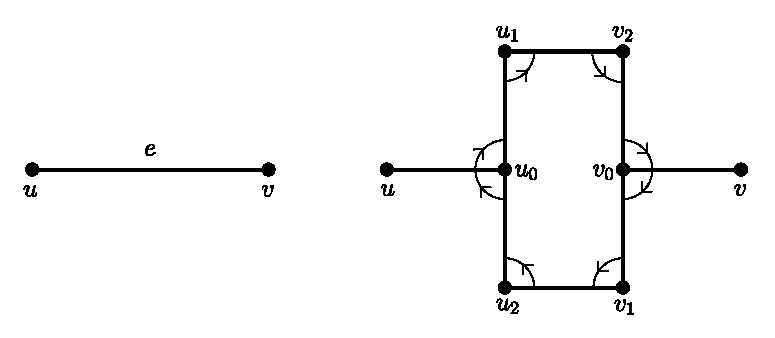
\includegraphics[width=.65\linewidth]{KernelMengerian-gadget}
  \caption{The gadget introduced for parallel edges}
  \label{gadget}
\end{figure}
such that $u u_0$ (\textit{resp.} $v v_0$) has the same order with $u v$ in $\prec_u$ (\textit{resp.} $\prec_v$).
Notice that the construction preserves the parity of cycles with cyclic preferences in $H$.

\begin{lemma}
\label{lem:reduct1}
$FSM(H,\prec)$ is a projection of $FSM(H^\prime,\prec^\prime)$.
\end{lemma}
\begin{proof}
Take $x\in FSM(H,\prec)$.
For each parallel edge $e$ with endpoints $u$ and $v$ in $H$,
we set the value of edges in the gadget corresponding to $e$ as follows:
\begin{enumerate}[label={(\alph*)}, itemsep=0.2mm]
  \item $x^\prime_{u u_0}=x^\prime_{v v_0}:=x_{e}$;
  \item $x^\prime_{u_0 u_1}=x^\prime_{v_0 v_2}:=1-x_{e}-x(\varphi_u(e))$;
  \item $x^\prime_{u_0 u_2}=x^\prime_{v_0 v_1}:=x(\varphi_u (e))$;
  \item $x^\prime_{u_1 v_2}:=x_e +x(\varphi_u (e))$;
  \item $x^\prime_{u_2 v_1}:=1-x(\varphi_u (e))$.
\end{enumerate}
For each edge $f$ without parallel edges in $H$, set $x^\prime_f:=x_f$.
It is easy to check that $x^\prime\in FSM(H^\prime, \prec^\prime)$.
Hence $FSM(H,\prec)$ is a projection of $FSM(H^\prime,\prec^\prime)$.
\end{proof}

By Theorem \ref{thm:AbelRoth94} and Lemma \ref{lem:reduct1}, $FSM(H,\prec)$ is $1/2$-integral since $FSM(H^\prime,\prec^\prime)$ is $1/2$-integral.
Hence vertices in $FSM(H,\prec)$ with $x(O)=3/2$ where $O\in \mathcal{O}(H)$ are the only possible vertices of $FSM(H,\prec)$ that violate constraints (\ref{constraints:4}).
However each $O$ with $x(O)=3/2$ leads to a $3$-cycle with cyclic preferences which arises from a directed $3$-cycle in $D$, contradicting to the assumption that $D$ is clique-acyclic.
It follows that constraints (\ref{constraints:4}) are unbinding for all vertices of $FSM(H,\prec)$.
Hence constraints (\ref{constraints:4}) are redundant with respect to $\pi(H,\prec)$

\begin{lemma}
\label{lem:reduct2}
  If $\pi(H^\prime,\prec^\prime)$ is  totally dual integral, then so is $\pi(H,\prec)$.
\end{lemma}
\begin{proof}
  We show that $\pi(H,\prec)$ can be obtained from $\pi(H^\prime,\prec^\prime)$ after a series of Fourier-Motzkin eliminations.
  It suffices to demonstrate one elimination process from a gadget to an edge.
  Given a gadget as in Figure \ref{gadget} arising from edge $e$, eliminate $u_1 v_2$ from $\pi(H^\prime,\prec^\prime)$ first.
  Then all constraints involving $x_{u_1 v_2}$ are replaced by equality $x_{u_0 u_1}=x_{v_0 v_2}$.
  Similarly, eliminating $u_2 v_1$ yields equality $x_{v_0 v_1}=x_{u_0 u_2}$.
  Next eliminating $u u_0$ gives $x(\delta (u)\backslash\{u u_0\})\leq x_{u_0 u_1}+x_{u_0 u_2}$ and $x_{u_0 u_2}\leq x(\varphi_u(uv))$.
  After eliminating $u_0 u_1$ and $u_0 u_2$, we arrive at $x(\delta(u)\backslash\{u u_0\})\leq x_{v_0 v_1}+x_{v_0 v_2}$ and $x_{v_0 v_1}\leq x(\varphi_u(uv))$.
  In the end, canceling $v_0 v_1$ and $v_0 v_2$ gives $x_{v v_0}+x(\varphi_v(v v_0)+x(\varphi_u(u u_0))\geq 1$ and $x_{v v_0}+x(\delta(u)\backslash\{u u_0\})\leq 1$.
  Besides, $x_{v v_0}+x(\delta(v)\backslash\{v v_0\})\leq 1$ is unchanged.
  Hence all constraints involving edges from the gadget are reduced to three constraints
  $x_{v v_0}+x(\varphi_v(v v_0)+x(\varphi_u(u u_0))\geq 1$,
  $x_{v v_0}+x(\delta (u)\backslash\{u u_0\})\leq 1$,
  and $x_{v v_0}+x(\delta(v)\backslash\{v v_0\})\leq 1$,
  which can be viewed as $x(\varphi(e))\geq 1$, $x(\delta(u))\leq 1$, and $x(\delta(v))\leq 1$ respectively.
  Performing Fourier-Motzkin eliminations in such an order for each gadget in $H^\prime$ leads to a linear system defined on $(H,\prec)$, which is precisely the same with $\pi(H,\prec)$ (renaming variables and removing duplicating constraints if necessary).
  As proved by Cook \cite{Cook83}, total dual integrality is preserved under Fourier-Motzkin elimination of a variable if it occurs in each constraint with coefficient $0$ or $\pm 1$.
  Hence the lemma follows.
\end{proof}

By Lemma \ref{lem:reduct1} and Lemma \ref{lem:reduct2}, we generalize the theorem of Chen \textit{et al.} \cite{ChenDing12} on the stable matching problem to multigraphs.
\begin{corollary}
  Let $(G,\prec)$ be a preference system, where $G$ is a multigraph.
  Then $\pi(G,\prec)$ is $1/2$-totally dual integral.
  Moreover, $\pi(G,\prec)$ is totally dual integral if and only if $FSM(G,\prec)=SM(G,\prec)$.
\end{corollary}

Moreover, we have the following corollary for kernels in clique-acyclic orientations of line multigraph.
\begin{corollary}
  Let $D$ be a clique-acyclic orientation of line multigraph.
  Then $\sigma(D)$ is $1/2$-totally dual integral.
  Moreover, $\sigma(D)$ is totally dual integral if and only if $FK(D)=K(D)$.
\end{corollary}

\section{Proofs}
Observe that when $D$ is good, both $(H,\prec)$ and $(H^\prime,\prec^\prime)$ admit no odd cycles with cyclic preferences.
In the following we exhibit some properties of simple preference systems admitting no odd cycles with cyclic preferences.
\begin{lemma}
\label{lem:prf1}
Let $(G,\prec)$ be a simple preference system. If $(G,\prec)$ admits no odd cycles with cyclic preferences, then $SM(G,\prec)=FSM(G,\prec)$.
\end{lemma}

By Theorem \ref{thm:ChenDing12}, integrality of $FSM(G,\prec)$ is equivalent to total dual integrality of $\pi(G,\prec)$, where $(G,\prec)$ is a simple preference system. A corollary follows directly.

\begin{corollary}
\label{cor:prf2}
Let $(G,\prec)$ be a simple preference system. If $(G,\prec)$ admits no odd cycles with cyclic preferences, then $\pi(G,\prec)$ is totally dual integral.
\end{corollary}

\begin{proof}[Proof of Lemma \ref{lem:prf1}]
By Theorem \ref{thm:AbelRoth94}, $FSM(G,\prec)$ is $1/2$-integral as $(G,\prec)$ is a simple preference system.
Let $x$ be a $1/2$-integral point in $FSM(G, \prec)$.
Since $(G,\prec)$ admits no odd cycles with cyclic preferences, $E_{1/2}(x)$ consists of even cycles $C_1,C_2,\ldots,C_r$ with cyclic preferences. For $i=1,2,\ldots,r$, label vertices and edges of $C_i\in E_{1/2}(x)$ such that $C_i=v^i_1v^i_2\ldots v^i_{l}$ and $e^i_k\prec_{v^i_{k+1}} e^i_{k+1}$ for $k=1,2,\ldots,l$, where $e^i_k=v^i_{k}v^i_{k+1}$ and indices are taken modulo $l$.
We remark that the parity of vertices and edges refers to the parity of their indices. Define $z\in \mathbb{R}^{E(G)}$ by
\begin{equation*}
z(e):=
\begin{cases}
1 & e\text{ is an even edge in }C \in E_{1/2}(x),\\
-1 & e\text{ is an odd edge in }C \in E_{1/2}(x),\\
0 & \text{otherwise}.
\end{cases}
\end{equation*}
We are going to exclude $x$ from vertices of $FSM(G, \prec)$ by adding perturbation $\epsilon z$ for small $\epsilon$ to $x$ and showing that $x\pm\epsilon z\in FSM(G,\prec)$.
Tight constraints in (\ref{stability constraints})-(\ref{edge nonnegativity}) under perturbation $\epsilon z$ play a key role here. Observe that tight constraints in (\ref{matching constraints}) and (\ref{edge nonnegativity}) are invariant under perturbation $\epsilon z$. It remains to show that perturbation $\epsilon z$ does not affect tight constraints in (\ref{stability constraints}) either. Let $e$ be an edge with $x(\varphi(e))=1$. Clearly, $\lvert \varphi(e)\cap E_+(x)\rvert \in\{1,2\}$. When $\lvert \varphi(e)\cap E_+(x)\rvert=1$, $x(e)=1$ follows, which is trivial. When $\lvert \varphi(e)\cap E_+(x)\rvert =2$, we claim that the parity of dominating edges in $E_{1/2}(x)$ of $e$ does not agree (relabeling vertices and edges in $E_{1/2}(x)$ if necessary).
Hence corresponding tight constraints in (\ref{stability constraints}) are also invariant under perturbation $\epsilon z$.
To justify this claim, we distinguish four cases.

\textbf{Case 1.} Edge $e$ is an edge from some $C\in E_{1/2}(x)$. This case is trivial since $C$ admits cyclic preferences.

\begin{figure}
\centering
\begin{subfigure}{.4\textwidth}
  \centering
  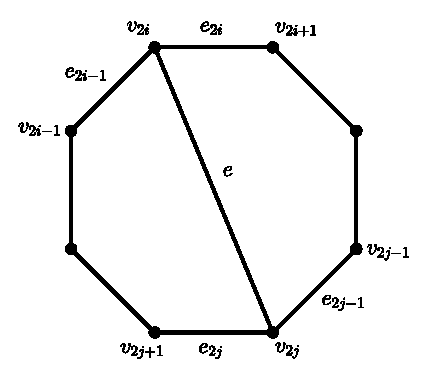
\includegraphics[width=.85\linewidth]{KernelMengerian-fig1a}
  \caption{}
  \label{fig1a}
\end{subfigure}%
\begin{subfigure}{.4\textwidth}
  \centering
  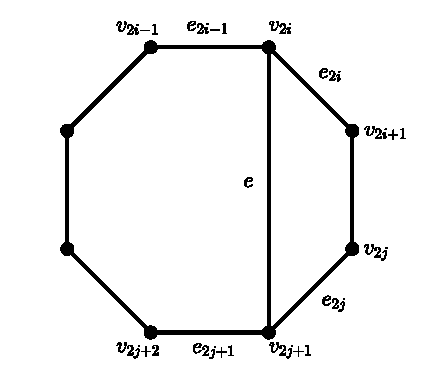
\includegraphics[width=.845\linewidth]{KernelMengerian-fig1b}
  \caption{}
  \label{fig1b}
\end{subfigure}
\caption{Case 2}
\end{figure}
\textbf{Case 2.} Edge $e$ is a chord in some $C\in E_{1/2}(x)$. We first show that endpoints of $e$ have different parity in $C$. We prove it by contradiction. Without loss of generality, let $e=v_{2i}v_{2j}$.

If $e_{2i}\prec e$, then $e_{2i-1}\prec e$. Since $x(\varphi(e))=1$, it follows that $e\prec e_{2j-1}$ and $e\prec e_{2j}$. However, $v_{2i} e v_{2j} e_{2j} v_{2j+1} \ldots v_{2i-1} e_{2i-1} v_{2i}$ form an odd cycle with cyclic preferences, a contradiction. Hence $e\prec e_{2i}$.

Similarly, if $e_{2j}\prec e$, then $e_{2j-1}\prec e$. Equality $x(\varphi(e))=1$ implies that $e\prec e_{2i}$ and $e\prec e_{2i-1}$. However, $v_{2i} e_{2i} v_{2i+1} \ldots v_{2j-1} e_{2j-1} v_{2j} e v_{2i}$ form an odd cycle with cyclic preferences, a contradiction. Hence $e\prec e_{2j}$.

Now $e\prec e_{2i}$ and $e\prec e_{2j}$, it follows that $e_{2i-1}\prec e$ and $e_{2j-1}\prec e$ since $x(\varphi(e))=1$. But in this case two odd cycles with cyclic preferences mentioned above occur at the same time.
Therefore, endpoints of $e$ have different parity in $C$. Hence let $e=v_{2i} v_{2j+1}$.
If $e_{2i}\prec e$ (\textit{resp.} $e_{2j+1}\prec e$), it follows that $e_{2i-1}\prec e$ (\textit{resp.} $e_{2j}\prec e$). Then $e$ is dominated by two consecutive edges from $C$, which is trivial.  So assume that $e\prec e_{2i}$ and $e\prec e_{2j+1}$. Since $x(\varphi(e))=1$, it follows that $e_{2i+1}\prec e$ and $e_{2j}\prec e$. Therefore e is dominated by two edges with different parity.

\textbf{Case 3.} Edge $e$ is a hanging edge of some $C\in E_{1/2}(x)$ and dominated by two edges from $C$. This case is trivial.

\begin{figure}
\centering
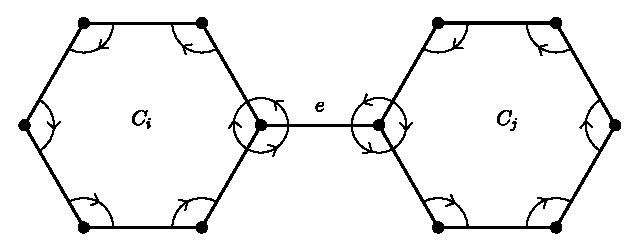
\includegraphics[scale=0.85]{KernelMengerian-fig2}
\caption{Case 4}
\end{figure}
\textbf{Case 4.} Edge $e$ is a connecting edge between $C_i$ and $C_j$ and dominated by one edge from $C_i$ and one edge from $C_j$ respectively, where $C_i, C_j \in E_{1/2}(x)$.
For $k=1,2,\ldots,r$, let $F_k$ be the subset of edges in this case and incident to $C_k$.
Then $\cup_{i=1}^{i=r} F_i\cup C_i$ induces a subgraph of $G$. It suffices to work on a component of the induced subgraph. We apply induction on the number $\alpha$ of cycles from $E_{1/2}(x)$ in a component.

When $\alpha=1$, it is trivial.
Hence assume the claim holds for components with $\alpha\geq 1$ cycles from $E_{1/2}(x)$. We consider a component with $\alpha +1$ cycles $C_1, \ldots, C_{\alpha}, C_{\alpha+1}$ from $E_{1/2}(x)$.
Without loss of generality, assume that deleting $C_{\alpha+1}$ yields a new component with $\alpha$ cycles.
By induction hypothesis, the claim holds for the resulting component.
It remains to check edges in $F_{\alpha+1}$. If there exists an edge in $F_{\alpha+1}$ violating the claim, relabel vertices and edges in $C_{\alpha+1}$. After at most one relabeling, all edges in $F_{\alpha+1}$ satisfy the claim. We prove it by contradiction. Let $f_1,f_2 \in F_{\alpha +1}$ be edges such that $f_1$ satisfies the claim but $f_2$ violates the claim. For $i=1,2$, let $f_i=u_i w_i$, where $u_i$ is the endpoint in the resulting component and $w_i$ is the endpoint in $C_{\alpha+1}$. By assumption, $u_1$ and $w_1$ have different parity and $u_2$ and $w_2$ have the same parity.
Analogous to the definition of cycles with cyclic preferences, we call path $P=v_1 v_2 \ldots v_l$ a \textit{$v_1 v_l$-path with linear preferences} if $v_iv_{i+1}\prec_{v_{i+1}}v_{i+1}v_{i+2}$ for $i=1,2,\ldots,l-2$. Clearly, for any two vertices in the same component, there exists a path with linear preferences between them.
Hence there exist a $u_1 u_2$-path $P_\alpha$ and a $w_2 w_1$-path $P_{\alpha+1}$, both of which admit linear preferences.
Moreover, $u_1 P_\alpha u_2 f_2 w_2 P_{\alpha+1} w_1 f_1 u_1$ form a cycle with cyclic preferences. We justify this cycle is odd by
showing that the $u_1 u_2$-path $P_\alpha$ is even (\textit{resp.} odd) if $u_1$ and $u_2$ have the same (\textit{resp.} different) parity.

If $u_1$ and $u_2$ belong to the same cycle from $E_{1/2}(x)$, it is trivial. Hence assume $u_1\in C_s$ and $u_2\in C_t$, where $s,t\in \{1,2,\ldots,\alpha\}$ and $s\not=t$. We apply induction on the number $\tau$ of cycles from $E_{1/2}(x)$ involved in $P_\alpha$. Clearly, $\tau\geq 2$.
When $\tau=2$. Take $v^s v^t\in F_s\cap F_t$ on $P_\alpha$.
Let $P_s$ be the part of $P_\alpha$ from $u_1$ to $v^s$ in $C_s$ and $P_t$ be the part of $P_\alpha$ from $v^t$ to $u_2$ in $C_t$.
It follows that $u_1 P_s v^s v^t P_t u_2$ form $P_\alpha$.
By primary induction hypothesis, $v^s$ and $v^t$ have different parity since $v^s v^t\in F_s\cap F_t$.
If $u_1$ and $u_2$ have the same parity, then $P_s$ and $P_t$ have different parity, implying that $P_\alpha$ is even; if $u_1$ and $u_2$ have different parity, then $P_s$ and $P_t$ have the same parity, implying that $P_\alpha$ is odd.
Now assume $\tau\geq 2$. Let $C_{k_1},\ldots,C_{k_\tau},C_{k_{\tau+1}}$ be cycles from $E_{1/2}(x)$ involved along $P_\alpha$.
Take $v^{k_{\tau}} v^{k_{\tau+1}} \in F_{k_{\tau}}\cap F_{k_{\tau+1}}$ on $P_\alpha$.
Let $P_{s, k_{\tau}}$ denote the part of $P_\alpha$ from $u_1$ to $v^{k_{\tau}}$ and $P_{k_{\tau},t}$ denote the part of $P_\alpha$ from $v^{k_{\tau}}$ to $u_2$.
Clearly, $P_\alpha=u_1 P_{s,k_\tau} v^{k_\tau} P_{k_\tau, t} u_2$. Since $P_{s, k_{\tau}}$ involves $\tau$ cycles and $P_{k_{\tau},t}$ involves two cycles, both length depend on the parity of endpoints. It follows that $P_\alpha$ is even when $u_1$ and $u_2$ have the same parity, and $P_\alpha$ is odd when $u_1$ and $u_2$ have different parity.

Hence when $u_1$ and $u_2$ have the same parity, $w_1$ and $w_2$ have different parity, implying that $P_\alpha$ is even and $P_{\alpha+1}$ is odd;
when $u_1$ and $u_2$ have different parity, $w_1$ and $w_2$ have the same parity, implying that $P_\alpha$ is odd and $P_{\alpha+1}$ is even.
Either case yields an odd cycle with cyclic preferences, a contradiction.

Therefore $1/2$-integral points are not vertices of $FSM(G,\prec)$ as they can be perturbed by $\epsilon z$ for small $\epsilon$ without leaving $FSM(G,\prec)$ . By Theorem \ref{thm:AbelRoth94}, $SM(G,\prec)=FSM(G,\prec)$ follows.
\end{proof}

Now we are ready to present a proof of our main theorem.

\begin{proof}[Proof of Theorem \ref{thm:main}]
It suffices to show the equivalence of $(i)$, $(iii)$ and $(iv)$. Let $D$ be a good orientation of line multigraph $L(H)$.
Construct preference system $(H,\prec)$ from $D$, and construct simple preference system $(H^\prime,\prec^\prime)$ from $(H,\prec)$ by substituting each parallel edge with a gadget as in Figure \ref{gadget}.
By the construction, $(H^\prime,\prec^\prime)$ admits no odd cycles with cyclic preferences.
Now $\sigma(D)$ can be viewed as a linear system defined on preference system $(H,\prec)$ and consisting of constraints (\ref{constraints:1})-(\ref{constraints:5}).
Observe that constraints (\ref{constraints:1}), (\ref{constraints:2}) and $(\ref{constraints:5})$ form the Rothblum system $\pi(H,\prec)$, and constraints (\ref{constraints:3})-(\ref{constraints:4}) are redundant with respect to $\pi(H,\prec)$.
Hence $FK(D)=FSM(H,\prec)$ follows.

By Lemma \ref{lem:prf1}, $FSM(H^\prime,\prec^\prime)$ is integral.
Integrality of $FSM(H,\prec)$ follows from Lemma \ref{lem:reduct1}, implying $FK(D)$ is integral.
Similar arguments apply to any induced subdigraphs of $D$. Hence $(i)\implies (iii)$.

By Corollary \ref{cor:prf2}, $\pi(H^\prime,\prec^\prime)$ is TDI.
Total dual integrality of $\pi(H,\prec)$ follows from Lemma \ref{lem:reduct2}.
Since $\pi(H,\prec)$ is part of $\sigma(D)$ and the other constraints (\ref{constraints:3})-(\ref{constraints:4}) are redundant in $\sigma(D)$ with respect to $\pi(H,\prec)$, total dual integrality of $\sigma(D)$ follows. Similar arguments apply to any induced subdigraphs of $D$. Hence $(iii)\implies (iv)$.

By a theorem of Edmonds and Giles \cite{EdmoGile77}, implication $(iv)\implies (iii)$ follows directly.

To prove implication $(iii)\implies (i)$, we assume the contrary.
Observe that $D$ being kernel ideal implies the existence of kernels for any induced subdigraphs of $D$.
Let $D$ be a digraph such that $D$ is kernel ideal but not good.
Then there either exists a clique containing directed cycles or exists a directed odd cycle without (pseudo-)chords.
We show that neither case is possible.
If $D$ has a clique containing directed cycles, we consider the subdigraph induced on this clique.
There is no kernel for this induced subdigraph, a contradiction.
If $D$ contains a directed odd cycle without (pseudo-)chords, we restrict ourselves to the subdigraph induced on this directed odd cycle.
There is no kernel for this induced subdigraph either, a contradiction.
\end{proof}

\section{Discussions}
It is natural to consider whether our result applies to superorientations of line multigraph.
However, the connection between kernels and stable matchings seems to be broken by superorientations.
Indeed, consider the digraph $D=(V,A)$, where $V=\{1,2,3,4\}$ and $A=\{(1,2),(2,1),(3,1),(3,4),(4,2)\}$.
Clearly, $D$ is a good superorientation of a $4$-cycle which is a line graph.
However we cannot construct a preference system with strict linear preferences from $D$ such that kernels in $D$ correspond to stable matchings in the preference system.
Besides, the fractional kernel polytope $FK(D)$ has three vertices $(1,0,0,1)$, $(1/2,1/2,0,1/2)$ and $(0,1,1,0)$ including a fractional one.

\section*{Acknowledgments}
The author is grateful to Prof. Wenan Zang for his valuable suggestions.

\bibliographystyle{siam}
\bibliography{KernelMengerian}
\nocite{Schr86}

\end{document}
